% Options for packages loaded elsewhere
\PassOptionsToPackage{unicode}{hyperref}
\PassOptionsToPackage{hyphens}{url}
%
\documentclass[
]{article}
\usepackage{amsmath,amssymb}
\usepackage{lmodern}
\usepackage{iftex}
\ifPDFTeX
  \usepackage[T1]{fontenc}
  \usepackage[utf8]{inputenc}
  \usepackage{textcomp} % provide euro and other symbols
\else % if luatex or xetex
  \usepackage{unicode-math}
  \defaultfontfeatures{Scale=MatchLowercase}
  \defaultfontfeatures[\rmfamily]{Ligatures=TeX,Scale=1}
\fi
% Use upquote if available, for straight quotes in verbatim environments
\IfFileExists{upquote.sty}{\usepackage{upquote}}{}
\IfFileExists{microtype.sty}{% use microtype if available
  \usepackage[]{microtype}
  \UseMicrotypeSet[protrusion]{basicmath} % disable protrusion for tt fonts
}{}
\makeatletter
\@ifundefined{KOMAClassName}{% if non-KOMA class
  \IfFileExists{parskip.sty}{%
    \usepackage{parskip}
  }{% else
    \setlength{\parindent}{0pt}
    \setlength{\parskip}{6pt plus 2pt minus 1pt}}
}{% if KOMA class
  \KOMAoptions{parskip=half}}
\makeatother
\usepackage{xcolor}
\IfFileExists{xurl.sty}{\usepackage{xurl}}{} % add URL line breaks if available
\IfFileExists{bookmark.sty}{\usepackage{bookmark}}{\usepackage{hyperref}}
\hypersetup{
  pdftitle={Forecast Similarity Using Cramer Distance Approximation},
  pdfauthor={Johannes Bracher, Evan Ray, Nick Reich, Nutcha Wattanachit},
  hidelinks,
  pdfcreator={LaTeX via pandoc}}
\urlstyle{same} % disable monospaced font for URLs
\usepackage[margin=1in]{geometry}
\usepackage{graphicx}
\makeatletter
\def\maxwidth{\ifdim\Gin@nat@width>\linewidth\linewidth\else\Gin@nat@width\fi}
\def\maxheight{\ifdim\Gin@nat@height>\textheight\textheight\else\Gin@nat@height\fi}
\makeatother
% Scale images if necessary, so that they will not overflow the page
% margins by default, and it is still possible to overwrite the defaults
% using explicit options in \includegraphics[width, height, ...]{}
\setkeys{Gin}{width=\maxwidth,height=\maxheight,keepaspectratio}
% Set default figure placement to htbp
\makeatletter
\def\fps@figure{htbp}
\makeatother
\setlength{\emergencystretch}{3em} % prevent overfull lines
\providecommand{\tightlist}{%
  \setlength{\itemsep}{0pt}\setlength{\parskip}{0pt}}
\setcounter{secnumdepth}{-\maxdimen} % remove section numbering
\usepackage{amsmath}
\usepackage{tabularx}
\usepackage{hyperref}
\usepackage{multicol}
\usepackage{longtable}
\usepackage{array}
\usepackage{multirow}
\usepackage{wrapfig}
\usepackage{float}
\usepackage{colortbl}
\usepackage{pdflscape}
\usepackage{tabu}
\usepackage{threeparttable}
\usepackage{threeparttablex}
\usepackage{makecell}
\usepackage{xcolor}
\usepackage{tikz}
\usepackage{pgfplots}
\ifLuaTeX
  \usepackage{selnolig}  % disable illegal ligatures
\fi

\title{Forecast Similarity Using Cramer Distance Approximation}
\author{Johannes Bracher, Evan Ray, Nick Reich, Nutcha Wattanachit}
\date{03/02/2021}

\begin{document}
\maketitle

\hypertarget{cramer-distance}{%
\section{Cramer Distance}\label{cramer-distance}}

Consider two predictive distributions \(F\) and \(G\). Their
\emph{Cramer distance} or \emph{integrated quadratic distance} is
defined as

\[
\text{CD}(F, G) = \int_{-\infty}^\infty(F(x) - G(x))^2 dx
\] where \(F(x)\) and \(G(x)\) denote the cumulative distribution
functions. It can also be written as \begin{equation}
\text{CD}(F, G) = \mathbb{E}_{F, G}|x - y| - 0.5 \left[\mathbb{E}_F|x - x'| + \mathbb{E}_G|y - y'| \right], \label{eq:formulation_expectations}
\end{equation} where \(x, x'\) are independent random variables
following \(F\) and \(y, y'\) are independent random variables following
\(G\). This formulation illustrates that the Cramer distance depends on
the shift between \(F\) and \(G\) (first term) and the variability of
both \(F\) and \(G\) (of which the two last expectations in above
equation are a measure).

The Cramer distance is the divergence associated with the continuous
ranked probability score (Thorarinsdottir 2013, Gneiting and Raftery
2007), which is defined by

\begin{align}
\text{CRPS}(F, y) &= \int_{-\infty}^\infty(F(x) - \mathbf{1}(x \geq y))^2 dx = ) \\
&= 2\int_0^1((\mathbf{1}(y \leq q^F_k)-\tau_k)(q^F_k-y) d\tau_k \label{eq:crps}
\end{align}

where y denotes the observed value. Indeed, it is a generalization of
the CRPS as it simplifies to the CRPS if one out of F and G is a
one-point distribution. Indeed, it is a generalization of the CRPS as it
simplifies to the CRPS if one out of \(F\) and \(G\) is a one-point
distribution. The Cramer distance is commonly used to measure the
similarity of forecast distributions (see Richardson et al 2020 for a
recent application).

\hypertarget{cramer-distance-approximation-for-equally-spaced-intervals}{%
\subsection{Cramer Distance Approximation for Equally-Spaced
Intervals}\label{cramer-distance-approximation-for-equally-spaced-intervals}}

Now assume that for each of the distributions \(F\) and \(G\) we only
know \(K\) quantiles at equally spaced levels
\(\tau_1 = 1/(K + 1), \tau_2 = 2/(K + 1), \dots, \tau_K = K/(K + 1)\).
Denote these quantiles by \(q^F_1 \leq q^F_1 \leq \dots \leq q^F_K\) and
\(q^G_1 \leq q^G_2 \leq \dots \leq q^G_K\), respectively. It is well
known that the CRPS can be approximated by an average of linear quantile
scores (Laio and Tamea 2007, Gneiting and Raftery 2007):
\begin{equation}
\text{CRPS}(F, y) \approx \frac{1}{K} \times \sum_{k = 1}^K 2\{\mathbf{1}(y \leq q^F_k) - k/(K + 1)\} \times (q^F_k - y).\label{eq:linear_quantile_scores}
\end{equation} This approximation is equivalent to the weighted interval
score (WIS) which is in use for evaluation of quantile forecasts at the
Forecast Hub, see Section 2.2 of Bracher et al (2021). This
approximation can be generalized to the Cramer distance as
\begin{equation}
\text{CD}(F, G) \approx \frac{1}{K(K + 1)}\sum_{i = 1}^K\sum_{j = 1}^K 2 \times \mathbf{1}\{(i \leq j \land q^F_i > q^G_j) \lor (i \geq j \land q^F_i < q^G_j)\} \times \left| q^F_i - q^G_j\right|. \label{eq:approx_cd}
\end{equation} This can be seen as a sum of penalties for
\textit{incompatibility} of predictive quantiles. Whenever the
predictive quantiles \(q_i^F\) and \(q_j^G\) are incompatible in the
sense that they imply \(F\) and \(G\) are different distributions
(because \(q_F^i > q_G^j\) despite \(i \leq j\) or vice versa), a
penalty \(\left| q^F_i - q^G_j\right|\) is added.

\hypertarget{cramer-distance-approximation-for-unequally-spaced-intervals}{%
\subsection{Cramer Distance Approximation for Unequally-Spaced
Intervals}\label{cramer-distance-approximation-for-unequally-spaced-intervals}}

Suppose we have quantiles \(q_{1}^F,...,q_{K}^F\) and
\(q_{1}^G,...,q_{K}^G\) at \(K\) probability levels
\(\tau_1,...,\tau_K\) (with \(\tau_1=0\)) from two distributions \(F\)
and \(G\). Define the combined vector of quantiles
\(q_1, . . . , q_{2K}\) by combining the vectors \(q_{1}^F,...,q_{K}^F\)
and \(q_{1}^G,...,q_{K}^G\) and sorting them in an ascending order. The
CRPS can be approximated as follows \begin{equation}
\text{CRPS}(F, y) \approx \frac{1}{K}\sum_{k = 1}^K 2\{\mathbf{1}(y \leq q^F_k)-\tau_k\} \times (q^F_k - y) .\label{eq:ls_unqe}
\end{equation}

This approximation can be generalized to the Cramer distance as
\begin{equation}
\text{CD}(F, G) \approx \frac{1}{K}\sum_{i = 1}^K\sum_{j = 1}^K 2 \times w_{ij} \times \mathbf{1}\{(i \leq j \land q^F_i > q^G_j) \lor (i \geq j \land q^F_i < q^G_j)\} \times \left| q^F_i - q^G_j\right|, \label{eq:approx_cd_uneq}
\end{equation}

where \(w_{ij}=|\tau_i-\tau_j|\) (the difference of the probability
levels). The details on how to go from \eqref{eq:approx_cd_uneq} to the
Riemann sums are still being worked out. Essentially, we can approximate
the Cramer distance by eliminating the tails of the integral to the left
of \(q_1\) and the right of \(q_{2K}\), and approximating the center via
a Riemann sum:

\begin{align}
\text{CD}(F,G) &=\int^\infty_{-\infty}{F(x)−G(x)}^2dx\\
&\approx \int^{q_{2K}}_{q_1}{F(x)−G(x)}^2dx\\
&=\sum^{2K-1}_{j=1}\int^{q_{j+1}}_{q_j}{F(x)−G(x)}^2dx
\end{align}

There are a variety of options that can be used for each term in this
sum, for instance:

\hypertarget{left-sided-riemann-sum-approximation}{%
\subsubsection{Left-sided Riemann sum
approximation}\label{left-sided-riemann-sum-approximation}}

\begin{align}
\text{CD}(F,G) &\approx\sum^{2K-1}_{j=1}\int^{q_{j+1}}_{q_j}{F(x)−G(x)}^2\\
&\approx\sum^{2K-1}_{j=1}\{\hat{F}(q_j)-\hat{G}(q_j)\}^2(q_{j+1}-q_{j})\\
\end{align}

Since \(q_j\in \{q_1, ..., q_{2K}\}\) belongs to either
\(q_{1}^F,...,q_{K}^F\) or \(q_{1}^G,...,q_{K}^G\), we can rewrite the
above approximation using \(\tau_1,...,\tau_K\) as follows

\begin{align}
\text{CD}(F,G) 
&\approx\sum^{2K-1}_{j=1}\{\hat{F}(q_j)-\hat{G}(q_j)\}^2(q_{j+1}-q_{j})\\
&=\sum^{2K-1}_{j=1}\{\tau^F_j-\tau^G_j\}^2(q_{j+1}-q_{j})
\end{align}

where \(\tau^F_j \in \boldsymbol{\tau_F}\) and
\(\tau^G_j \in \boldsymbol{\tau_G}\). \(\boldsymbol{\tau_F}\) and
\(\boldsymbol{\tau_G}\) are vectors of length \(2K-1\) with elements

\[
\tau^F_j=
\begin{cases}
I(q_1=q_1^F)\times \tau_{q_1}^F\hspace{7cm}\text{for }j=1\\
I(q_j\in \{q_1^F, ..., q_{K}^F\})\times \tau_{q_j}^F+I(q_j\in \{q_1^G, ..., q_{K}^G\})\times \tau_{j-1}^F\hspace{0.3cm}\text{for }j>1\\
\end{cases}
\]

where \(\tau_{q_j}^F\) is the probability level corresponding to \(q_j\)
given \(q_j\) in the pooled quantiles comes from \(F\), and
\(\tau_{j-1}^F\) is the \((j-1)^{th}\) probability level in
\(\boldsymbol{\tau_F}\).

\[
\tau^G_j=
\begin{cases}
I(q_1=q_1^G)\times \tau_{q_1}^G\hspace{7cm}\text{for }j=1\\
I(q_j\in \{q_1^G, ..., q_{K}^G\})\times \tau_{q_j}^G+I(q_j\in \{q_1^F,...,q_{K}^F\})\times \tau_{j-1}^G\hspace{0.3cm}\text{for }j>1\\
\end{cases}
\]

where \(\tau_{q_j}^G\) is the probability level corresponding to \(q_j\)
given \(q_j\) in the pooled quantiles comes from \(G\), and
\(\tau_{j-1}^G\) is the \((j-1)^{th}\) probability level in
\(\boldsymbol{\tau_G}\).

\hypertarget{trapezoidal-rule}{%
\subsubsection{Trapezoidal rule}\label{trapezoidal-rule}}

\begin{align}
\text{CD}(F,G) &\approx\sum^{2K-1}_{j=1}\int^{q_{j+1}}_{q_j}{F(x)−G(x)}^2\\
&\approx\sum^{2K-1}_{j=1}\frac{\{\hat{F}(q_j)-\hat{G}(q_j)\}^2+\{\hat{F}(q_{j+1})-\hat{G}(q_{j+1})\}^2}{2}(q_{j+1}-q_{j})\\
\end{align}

Similarly, we can rewrite the above approximation using
\(\tau_1,...,\tau_K\) as defined in the left-sided Riemann sum
approximation as follows

\begin{align}
\text{CD}(F,G) 
&\approx\sum^{2K-1}_{j=1}\frac{\{\hat{F}(q_j)-\hat{G}(q_j)\}^2+\{\hat{F}(q_{j+1})-\hat{G}(q_{j+1})\}^2}{2}(q_{j+1}-q_{j})\\
&=
\sum^{2K-1}_{j=1}\frac{\{\tau^F_j-\tau^G_j\}^2+\{\tau^F_{j+1}-\tau^G_{j+1}\}^2}{2}(q_{j+1}-q_{j}).
\end{align}

\hypertarget{cramer-distance-approximation-for-unequally-spaced-intervals-and-different-probability-levels}{%
\subsection{Cramer Distance Approximation for Unequally-Spaced Intervals
and Different Probability
Levels}\label{cramer-distance-approximation-for-unequally-spaced-intervals-and-different-probability-levels}}

We (probably) can further modify the formula of the Cramer distance
approximation for unequally-spaced intervals to accommodate different
probability levels from \(F\) and \(G\). Suppose we have quantiles
\(q_{1}^F,...,q_{N}^F\) at \(K\) probability levels
\(\tau_1^F,...,\tau_N^F\) from the distribution \(F\), and
\(q_{1}^G,...,q_{M}^G\) at \(M\) probability levels
\(\tau_1^G,...,\tau_M^G\) from the distribution \(G\). Define the
combined vector of quantiles \(q_1, . . . , q_{N+M}\) by combining the
vectors \(q_{1}^F,...,q_{N}^F\) and \(q_{1}^G,...,q_{M}^G\) and again
sorting them in an ascending order. Using the same definitions as
previously defined, we can approximate the Cramer distance via a Riemann
sum as follows:

\hypertarget{left-sided-riemann-sum-approximation-1}{%
\subsubsection{Left-sided Riemann sum
approximation}\label{left-sided-riemann-sum-approximation-1}}

\begin{align}
\text{CD}(F,G) &\approx\sum^{N+M-1}_{j=1}\int^{q_{j+1}}_{q_j}{F(x)−G(x)}^2\\
&\approx\sum^{N+M-1}_{j=1}\{\hat{F}(q_j)-\hat{G}(q_j)\}^2(q_{j+1}-q_{j}),\\
\end{align}

which we can rewrite using \(\tau_1^F,...,\tau_N^F\) and
\(\tau_1^G,...,\tau_M^G\) as follows

\begin{align}
\text{CD}(F,G) 
&\approx\sum^{N+M-1}_{j=1}\{\hat{F}(q_j)-\hat{G}(q_j)\}^2(q_{j+1}-q_{j})\\
&=\sum^{N+M-1}_{j=1}\{\tau^F_j-\tau^G_j\}^2(q_{j+1}-q_{j})
\end{align}

where \(\tau^F_j \in \boldsymbol{\tau_F}\) and
\(\tau^G_j \in \boldsymbol{\tau_G}\). \(\boldsymbol{\tau_F}\) and
\(\boldsymbol{\tau_G}\) are vectors of length \(N+M-1\) with elements

\[
\tau^F_j=
\begin{cases}
\tau_{q_j}^F\hspace{2cm}\text{if }q_j\in \{q_1^F, ..., q_{N}^F\}\\
\tau_{q_{j-1}}^F\hspace{1.8cm}\text{if }q_j\notin \{q_1^F, ..., q_{N}^F\}\\
\end{cases}
\]

where \(\tau_{q_j}^F\) is the probability level corresponding to \(q_j\)
given \(q_j\) in the pooled quantiles comes from \(F\).

\[
\tau^G_j=
\begin{cases}
\tau_{q_j}^G\hspace{2cm}\text{if }q_j\in \{q_1^G, ..., q_{M}^G\}\\
\tau_{q_{j-1}}^G\hspace{1.8cm}\text{if }q_j\notin \{q_1^G, ..., q_{M}^G\}\\
\end{cases}
\]

where \(\tau_{q_j}^G\) is the probability level corresponding to \(q_j\)
given \(q_j\) in the pooled quantiles comes from \(G\).

\hypertarget{trapezoidal-rule-1}{%
\subsubsection{Trapezoidal rule}\label{trapezoidal-rule-1}}

\begin{align}
\text{CD}(F,G) &\approx\sum^{2K-1}_{j=1}\int^{q_{j+1}}_{q_j}{F(x)−G(x)}^2\\
&\approx\sum^{N+M-1}_{j=1}\frac{\{\hat{F}(q_j)-\hat{G}(q_j)\}^2+\{\hat{F}(q_{j+1})-\hat{G}(q_{j+1})\}^2}{2}(q_{j+1}-q_{j}),\\
\end{align}

which we can rewrite as follows

\begin{align}
\text{CD}(F,G) 
&\approx\sum^{N+M-1}_{j=1}\frac{\{\hat{F}(q_j)-\hat{G}(q_j)\}^2+\{\hat{F}(q_{j+1})-\hat{G}(q_{j+1})\}^2}{2}(q_{j+1}-q_{j})\\
&=
\sum^{N+M-1}_{j=1}\frac{\{\tau^F_j-\tau^G_j\}^2+\{\tau^F_{j+1}-\tau^G_{j+1}\}^2}{2}(q_{j+1}-q_{j}).
\end{align}

\hypertarget{examples}{%
\section{Examples}\label{examples}}

\hypertarget{first-example}{%
\subsection{First example}\label{first-example}}

\begin{center}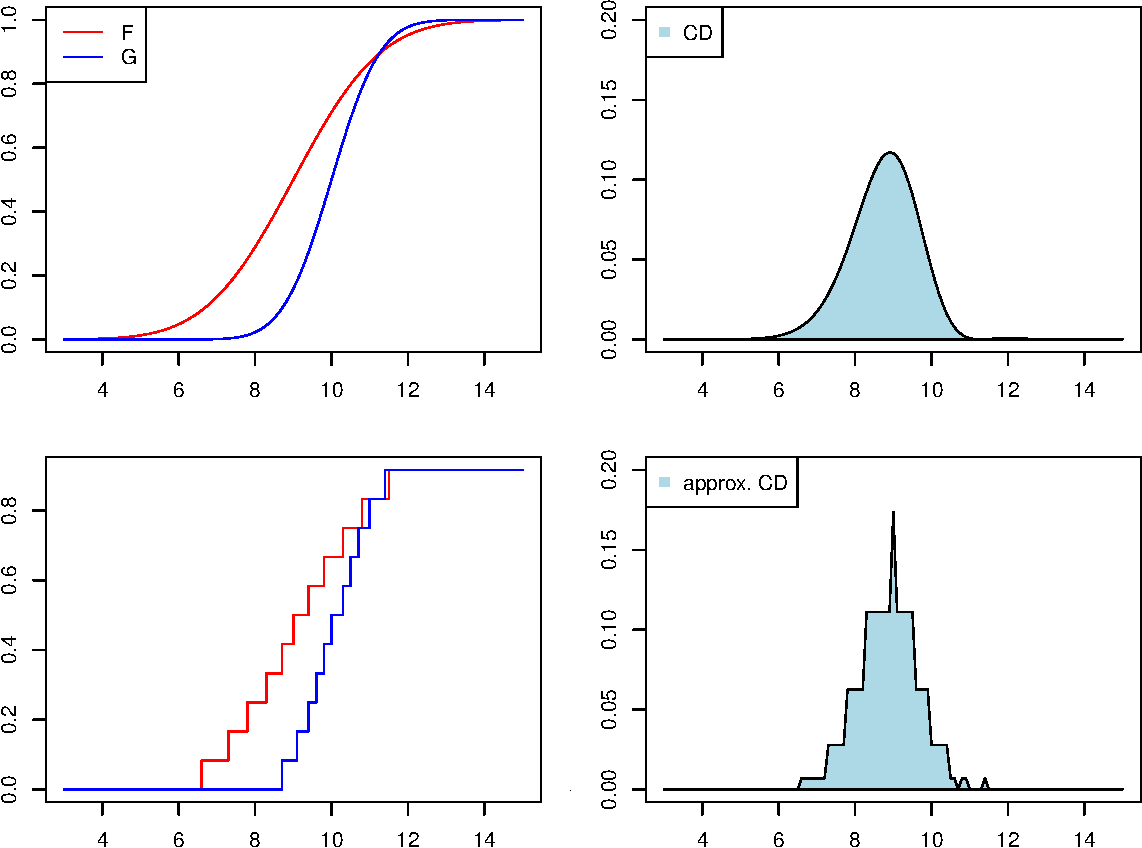
\includegraphics{cd_approx_2_files/figure-latex/ex1-1} \end{center}

In this example, six different approximations are applied to the
distributions \(F~N(9, 1.8)\) and \(G~N(10, 1)\) in the figures above.

\begin{itemize}
\tightlist
\item
  Using direct numerical integration based on a fine grid of values for
  \(x\):
\end{itemize}

\begin{verbatim}
FALSE [1] 0.2532376
\end{verbatim}

\begin{itemize}
\tightlist
\item
  Using the left-sided Riemann sum approximation and various values of
  \(K\):
\end{itemize}

\begin{verbatim}
FALSE  [1] 0.2324025 0.2296905 0.2339984 0.2353651 0.2343136 0.2370715 0.2390280
FALSE  [8] 0.2394081 0.2415779 0.2427410 0.2430888 0.2441036 0.2446913 0.2448760
FALSE [15] 0.2452973 0.2458022 0.2461450 0.2466688 0.2468641 0.2470812 0.2475265
\end{verbatim}

The below plot shows the results from the different computations.

\begin{center}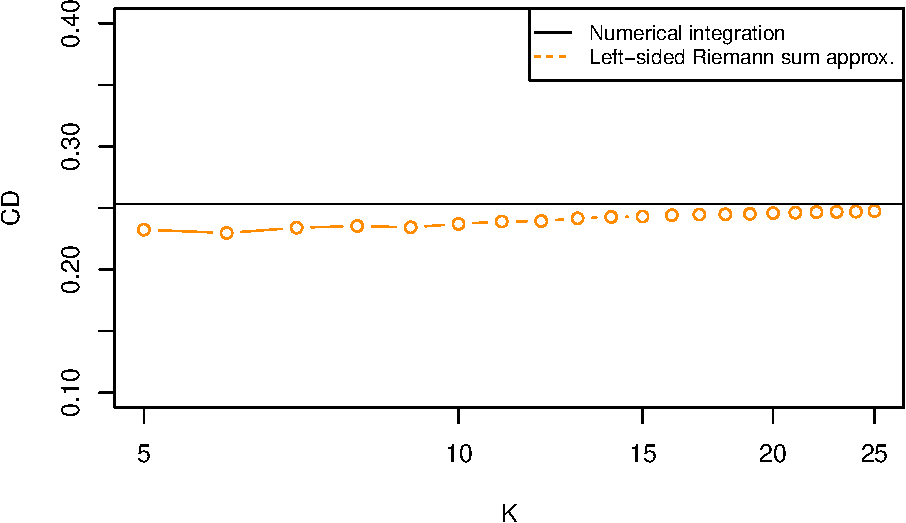
\includegraphics{cd_approx_2_files/figure-latex/unnamed-chunk-7-1} \end{center}

\hypertarget{second-example}{%
\subsection{Second example}\label{second-example}}

\begin{center}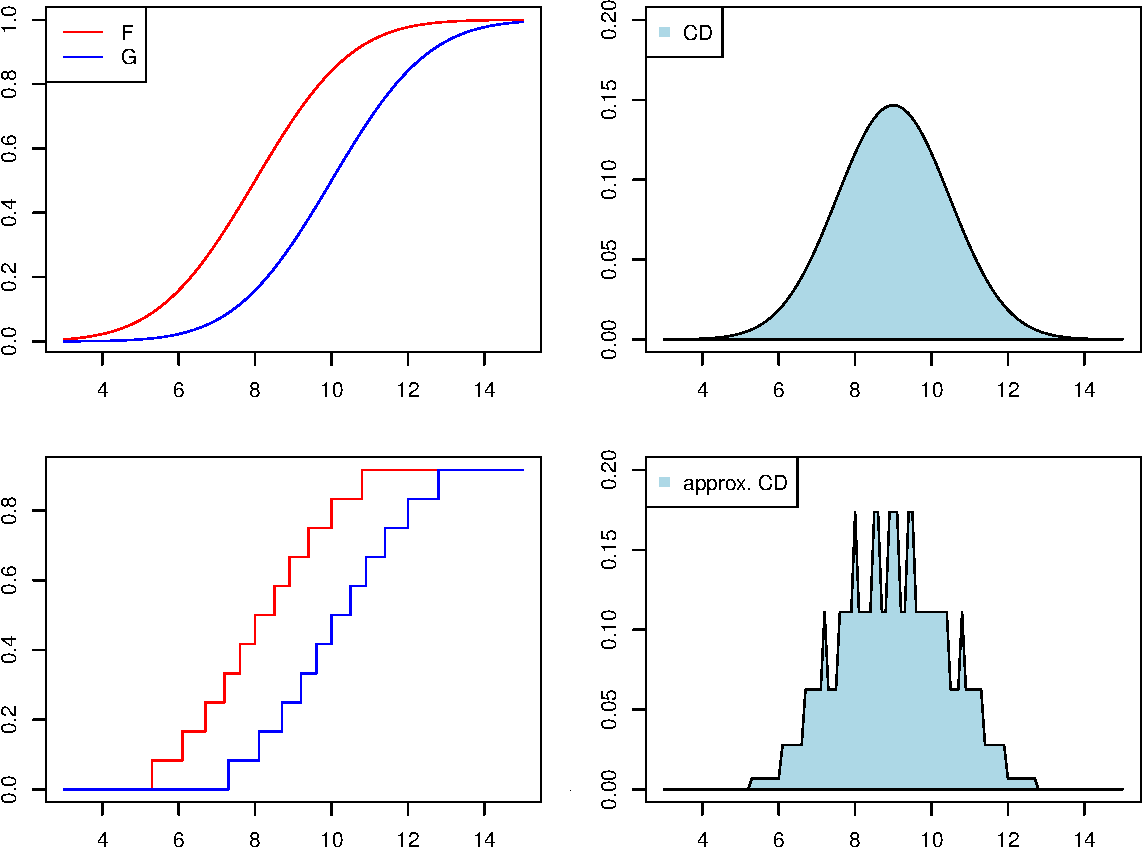
\includegraphics{cd_approx_2_files/figure-latex/ex2-1} \end{center}

\begin{itemize}
\tightlist
\item
  Using direct numerical integration based on a fine grid of values for
  \(x\):
\end{itemize}

\begin{verbatim}
FALSE [1] 0.5417857
\end{verbatim}

\begin{itemize}
\tightlist
\item
  Using the left-sided Riemann sum approximation and various values of
  \(K\):
\end{itemize}

\begin{verbatim}
FALSE  [1] 0.5306812 0.5298732 0.5385976 0.5352103 0.5391469 0.5380725 0.5368347
FALSE  [8] 0.5393677 0.5393195 0.5401040 0.5402759 0.5393039 0.5399378 0.5400548
FALSE [15] 0.5401662 0.5406499 0.5401523 0.5406339 0.5408435 0.5408465 0.5410123
\end{verbatim}

The below plot shows the results from the different computations.

\begin{center}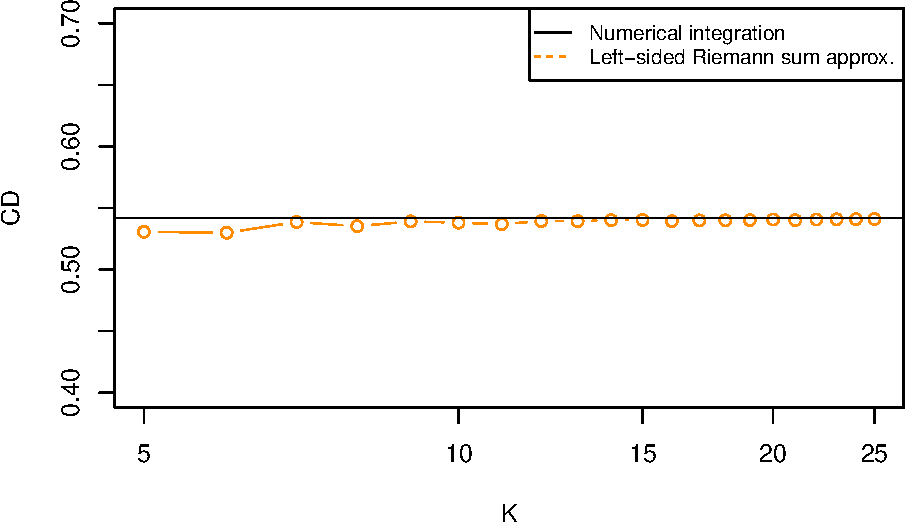
\includegraphics{cd_approx_2_files/figure-latex/unnamed-chunk-11-1} \end{center}

\hypertarget{third-example}{%
\subsection{Third example}\label{third-example}}

\begin{center}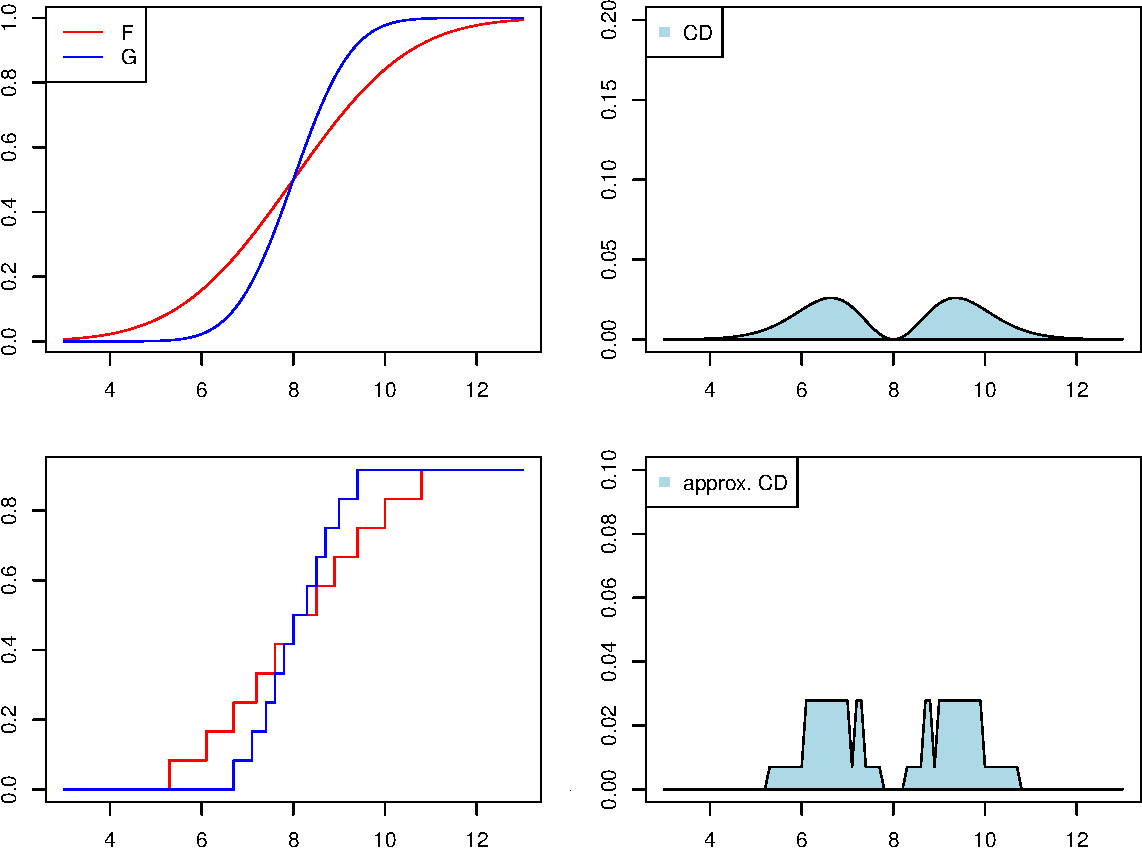
\includegraphics{cd_approx_2_files/figure-latex/ex3-1} \end{center}

\begin{itemize}
\tightlist
\item
  Using direct numerical integration based on a fine grid of values for
  \(x\):
\end{itemize}

\begin{verbatim}
FALSE [1] 0.09153308
\end{verbatim}

\begin{itemize}
\tightlist
\item
  Using the left-sided Riemann sum approximation and various values of
  \(K\):
\end{itemize}

\begin{verbatim}
FALSE  [1] 0.08759747 0.07767494 0.07927290 0.07939809 0.08313174 0.08237324
FALSE  [7] 0.08366803 0.08203895 0.08292167 0.08352577 0.08481403 0.08497727
FALSE [13] 0.08557163 0.08514638 0.08532199 0.08553263 0.08634072 0.08652439
FALSE [19] 0.08687125 0.08680405 0.08689452
\end{verbatim}

The below plot shows the results from the different computations.

\begin{center}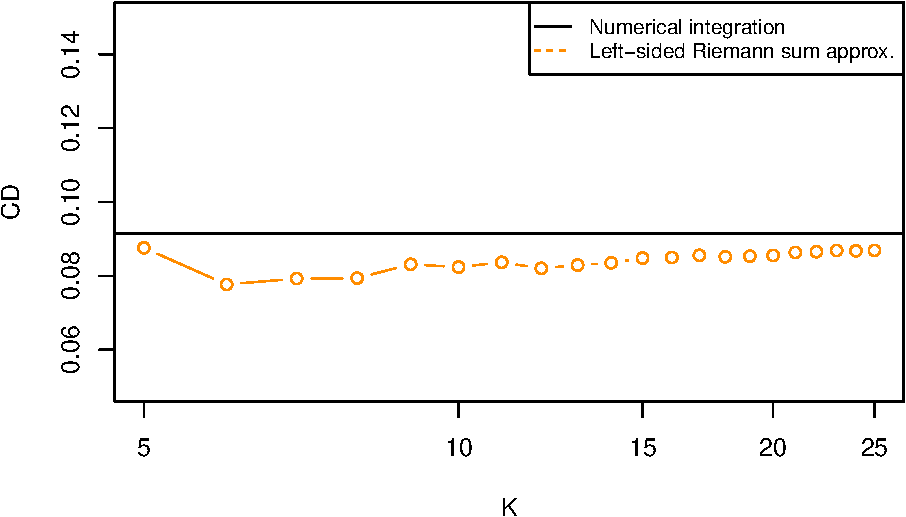
\includegraphics{cd_approx_2_files/figure-latex/unnamed-chunk-15-1} \end{center}

\hypertarget{make-a-plot-of-all-differences-between-real-vs-approx-for-all-cases}{%
\section{make a plot of all differences between real vs approx for all
cases}\label{make-a-plot-of-all-differences-between-real-vs-approx-for-all-cases}}

\begin{center}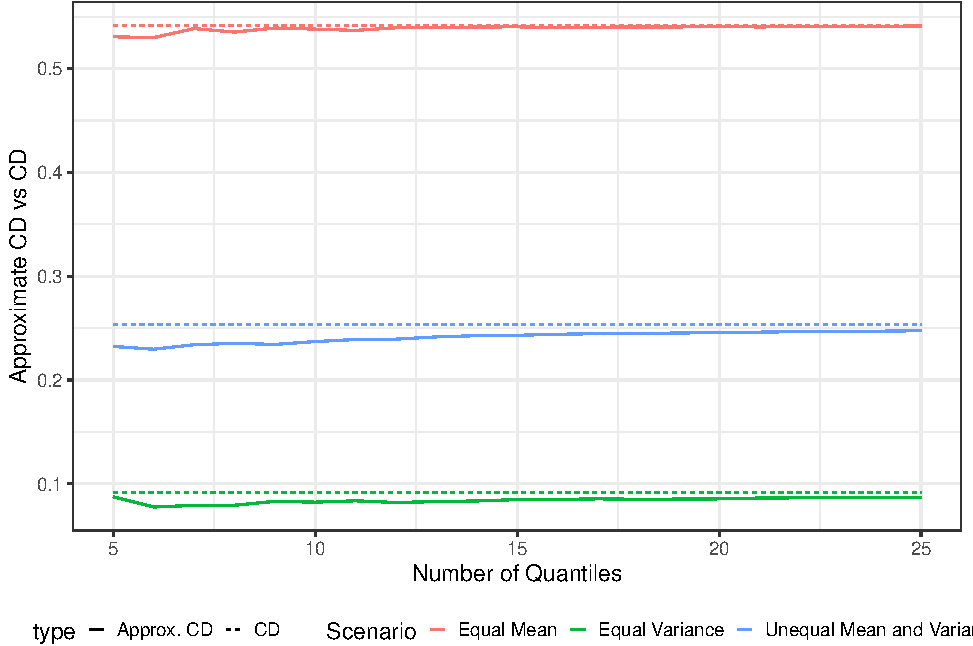
\includegraphics{cd_approx_2_files/figure-latex/diff-1} \end{center}

\begin{center}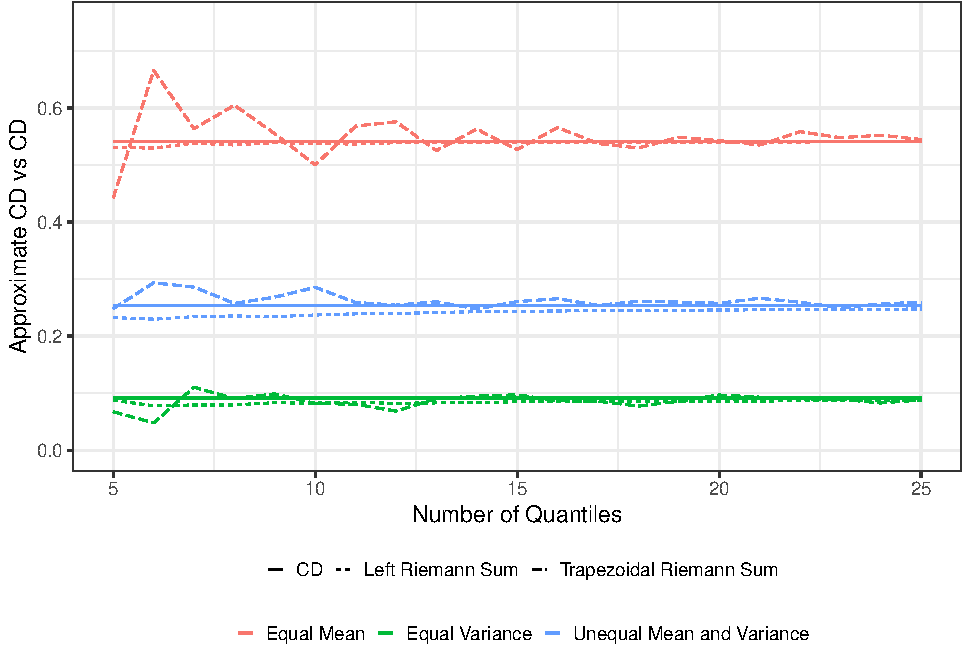
\includegraphics{cd_approx_2_files/figure-latex/diff2-1} \end{center}

\hypertarget{r-plot-plotvalues_k-cd_approx1-ylim-c0-0.5-xlab-k-ylab-cd-pch-1-type-b-log-x-col-darkorange-plotvalues_k-cd_approx31-ylim-c0.1-0.4-xlab-k-ylab-cd-pch-1-type-b-log-x-col-darkorange-linesvalues_k-cd_approx2-type-b-col-darkgreen-linesvalues_k-cd_approx3-type-b-col-blue-linesvalues_k-cd_approx4-type-b-col-brown-ablineh-cd_grid-col-black-ablineh-cd_sample-col-purple-lty-2-legendtopright-cgrid-based-sample-based-quantile-approx.-1-quantile-approx.-2-uneq-quantile-approx.-1-uneq-quantile-approx.-2-cgrid-based-sample-based-left-sided-riemann-sum-approx.-pch-cna-na-1-1-1-1-lty-c1-2-na-nana-na-pch-cna-na-1-lty-c1-2-na-col-cblack-purple-darkorange-darkgreenbluebrown-col-cblack-purple-darkorange-cex0.8}{%
\section{\texorpdfstring{\texttt{\{r\}\ \#\ \#\ plot:\ \#\ \#\ plot(values\_K,\ cd\_approx1,\ ylim\ =\ c(0,\ 0.5),\ xlab\ =\ "K",\ ylab\ =\ "CD",\ \#\ \#\ \ \ \ \ \ pch\ =\ 1,\ type\ =\ "b",\ log\ =\ "x",\ col\ =\ "darkorange")\ \#\ plot(values\_K,\ cd\_approx31,\ ylim\ =\ c(0.1,\ 0.4),\ xlab\ =\ "K",\ ylab\ =\ "CD",\ \#\ \ \ \ \ \ pch\ =\ 1,\ type\ =\ "b",\ log\ =\ "x",\ col\ =\ "darkorange")\ \#\ \#\ lines(values\_K,\ cd\_approx2,\ type\ =\ "b",\ col\ =\ "darkgreen")\ \#\ \#\ lines(values\_K,\ cd\_approx3,\ type\ =\ "b",\ col\ =\ "blue")\ \#\ \#\ lines(values\_K,\ cd\_approx4,\ type\ =\ "b",\ col\ =\ "brown")\ \#\ abline(h\ =\ cd\_grid,\ col\ =\ "black")\ \#\ abline(h\ =\ cd\_sample,\ col\ =\ "purple",\ lty\ =\ 2)\ \#\ legend("topright",\ \#\ \ \ \ \ \ \ \ \#\ c("grid-based",\ "sample-based",\ "quantile\ approx.\ 1",\ "quantile\ approx.\ 2",\ \#\ \ \ \ \ \ \ \ \#\ \ \ "uneq\ quantile\ approx.\ 1",\ "uneq\ quantile\ approx.\ 2"),\ \#\ \ \ \ \ \ \ \ c("grid-based",\ "sample-based",\ "left-sided\ Riemann\ sum\ approx."),\ \#\ \ \ \ \ \ \ \ \#\ pch\ =\ c(NA,\ NA,\ 1,\ 1,\ 1,\ 1),\ lty\ =\ c(1,\ 2,\ NA,\ NA,NA,\ NA),\ \#\ \ \ \ \ \ \ \ pch\ =\ c(NA,\ NA,\ 1),\ lty\ =\ c(1,\ 2,\ NA),\ \#\ \ \ \ \ \ \ \ \#\ col\ =\ c("black",\ "purple",\ "darkorange",\ "darkgreen","blue","brown"),\ \#\ \ \ \ \ \ \ \ col\ =\ c("black",\ "purple",\ "darkorange"),\ \#\ \ \ \ \ \ \ \ cex=0.8)\ \#}}{\{r\} \# \# plot: \# \# plot(values\_K, cd\_approx1, ylim = c(0, 0.5), xlab = "K", ylab = "CD", \# \#      pch = 1, type = "b", log = "x", col = "darkorange") \# plot(values\_K, cd\_approx31, ylim = c(0.1, 0.4), xlab = "K", ylab = "CD", \#      pch = 1, type = "b", log = "x", col = "darkorange") \# \# lines(values\_K, cd\_approx2, type = "b", col = "darkgreen") \# \# lines(values\_K, cd\_approx3, type = "b", col = "blue") \# \# lines(values\_K, cd\_approx4, type = "b", col = "brown") \# abline(h = cd\_grid, col = "black") \# abline(h = cd\_sample, col = "purple", lty = 2) \# legend("topright", \#        \# c("grid-based", "sample-based", "quantile approx. 1", "quantile approx. 2", \#        \#   "uneq quantile approx. 1", "uneq quantile approx. 2"), \#        c("grid-based", "sample-based", "left-sided Riemann sum approx."), \#        \# pch = c(NA, NA, 1, 1, 1, 1), lty = c(1, 2, NA, NA,NA, NA), \#        pch = c(NA, NA, 1), lty = c(1, 2, NA), \#        \# col = c("black", "purple", "darkorange", "darkgreen","blue","brown"), \#        col = c("black", "purple", "darkorange"), \#        cex=0.8) \#}}\label{r-plot-plotvalues_k-cd_approx1-ylim-c0-0.5-xlab-k-ylab-cd-pch-1-type-b-log-x-col-darkorange-plotvalues_k-cd_approx31-ylim-c0.1-0.4-xlab-k-ylab-cd-pch-1-type-b-log-x-col-darkorange-linesvalues_k-cd_approx2-type-b-col-darkgreen-linesvalues_k-cd_approx3-type-b-col-blue-linesvalues_k-cd_approx4-type-b-col-brown-ablineh-cd_grid-col-black-ablineh-cd_sample-col-purple-lty-2-legendtopright-cgrid-based-sample-based-quantile-approx.-1-quantile-approx.-2-uneq-quantile-approx.-1-uneq-quantile-approx.-2-cgrid-based-sample-based-left-sided-riemann-sum-approx.-pch-cna-na-1-1-1-1-lty-c1-2-na-nana-na-pch-cna-na-1-lty-c1-2-na-col-cblack-purple-darkorange-darkgreenbluebrown-col-cblack-purple-darkorange-cex0.8}}

\end{document}
